\documentclass[a4paper]{scrbook}


\usepackage[resetfonts]{cmap}

\usepackage{scrlayer-scrpage}
\lehead{Milet-Bibliographie}
\rohead{Stand: \today}

\usepackage{graphicx}
\usepackage{fontspec}
\usepackage[ngerman, shorthands=off]{babel}
\usepackage{xcolor}
\usepackage[style=german]{csquotes} 
\usepackage{textalpha}
\usepackage{array}

\definecolor{uhhred}{HTML}{E2001A}
\definecolor{uhhgrey}{HTML}{3b515b}

\usepackage[colorlinks = true, linkcolor = black, urlcolor  = uhhgrey]{hyperref}

%\setmainfont{CMU Sans}
\usepackage[default, scale=0.95]{sourcesanspro}

\usepackage[backend=biber, style=archaeologie, lstabbrv, sorting=nyt, maxcitenames=99, maxbibnames=99, maxnames=99]{biblatex}
\addbibresource{../data/Milet_Bibliography_BibLaTeX.bib}

%\renewcommand*{\mkbibnamefamily}[1]{\textsc{#1}}

\defbibenvironment{compactbib}
  {\list
     {}
     {\setlength{\leftmargin}{\bibhang}%
      \setlength{\itemindent}{-\leftmargin}%
      \setlength{\itemsep}{\bibitemsep}%
      \setlength{\parsep}{\bibparsep}}}
  {\endlist}
  {\item}

\renewcommand{\thesection}{\arabic{section}}

\newcommand{\redhref}[2]{\href{#1}{\color{uhhred}{#2}}}



\begin{document}

%\begin{figure}
%\includegraphics[width=\textwidth]{titel-stadtzentrum-desktop.png}
%\end{figure}
\begin{titlepage}
    \vspace*{3cm}
\begin{center}
    {\LARGE \textsc{\textbf{Milet-Bibliographie}}}\\
    
    Stand: \today
\end{center}
\vspace*{3cm}
\begin{figure}[h]
    \includegraphics[width=\textwidth]{Abb/Gelände2.png}
\end{figure}

\end{titlepage}

\thispagestyle{empty}
\section*{Verantwortliche}

Diese Bibliographie wurde von Sabine Huy im Rahmen ihrer Tätigkeit für das Miletarchiv begründet und bis 2022 in dieser Form als \redhref{https://doi.org/10.25592/uhhfdm.8678}{PDF-Version zum Download} angeboten. Unter Mitarbeit von Caitlin Bamford und Silas Munnecke wurde die Liste zum Jahr 2022 in eine Datenbankversion überführt und wird seitdem von Lisa Steinmann gepflegt. Die Bearbeitung und Verwaltung der Bibliographie erfolgt in einer \redhref{https://www.zotero.org/groups/4475959/milet_bibliography}{öffentlich zugänglichen Zotero-Gruppenbibliothek}. Dieses Dokument ist ein Export der Bibliographie, die in durchsuchbarer Form auch auf der \redhref{https://www.miletgrabung.uni-hamburg.de/material/bibliographie.html}{Homepage der Miletgrabung} zur Verfügung steht. Dort gibt es ebenfalls die Möglichkeit, die Bibliographie in diversen Formaten für den Import in Literaturverwaltungsprogramme herunterzuladen.\\

The bibliography has been offered as a \redhref{https://doi.org/10.25592/uhhfdm.8678}{PDF version for download} for many years by Sabine Huy in the course of her work at the Miletus Archive. With the collaboration of Caitlin Bamford and Silas Munnecke, the list was converted into a database version as of 2022 and has since been maintained by Lisa Steinmann. The bibliography is edited and managed in a \redhref{https://www.zotero.org/groups/4475959/milet_bibliography}{publicly accessible Zotero group library}. This document is an export of the bibliography, which is also available in searchable form on the \redhref{https://www.miletgrabung.uni-hamburg.de/material/bibliographie.html}{homepage of the Miletus Excavation}. There is also an option there to download the bibliography in various formats for import into literature management software. 

\vfill
\begin{tabular}{m{0.1\textwidth}  m{0.4\textwidth}}

\includegraphics[width=0.09\textwidth]{Abb/Logo.png} & 
\redhref{https://www.miletgrabung.uni-hamburg.de}{www.miletgrabung.uni-hamburg.de} 
\redhref{mailto:miletgrabung@uni-hamburg.de}{miletgrabung@uni-hamburg.de}\\
\end{tabular}

\newpage
\pagenumbering{Roman}
\tableofcontents

\chapter*{Milet-Bibliographie}
\nocite{*}
\pagenumbering{arabic}
\setcounter{page}{1}

Die folgende Bibliographie wird laufend ergänzt. Obwohl wir uns um eine Aufnahme aller Beiträge bemühen können wir die Vollständigkeit nicht garantieren. Über Ergänzungen und Korrekturhinweise sind wir jederzeit sehr dankbar. Falls Sie einen Beitrag zu Milet veröffentlichen oder veröffentlicht haben melden Sie sich gerne bei uns. Wir würden uns neben einem Eintrag in dieser Bibliographie auch sehr darüber freuen, Ihre Arbeit in digitaler Form in das Literaturarchiv der Miletgrabung aufzunehmen, das allen Wissenschaftler*innen in Milet vor Ort als Arbeitsbibliothek zur Verfügung steht. \\

The following bibliography is continuously updated. Although we put in every effort to include all contributions, we cannot guarantee completeness. We are always grateful for additions and corrections. If you are currently publishing or have published an article on Miletus, please contact us. In addition to an entry in this bibliography, we would also be very pleased to include your work in digital form in the literature archive of the Miletus excavation, which is available to all scholars at Miletus as a working library. 

\begin{flushleft}%
Sie erreichen uns unter / You can contact us at \redhref{mailto:miletgrabung@uni-hamburg.de}{miletgrabung@uni-hamburg.de}.
\end{flushleft}%
%\bibliographystyle{plain}
%\printbibheading
%\begin{flushleft}
%\section{Grabungs- und Arbeitsberichte}


\vfill
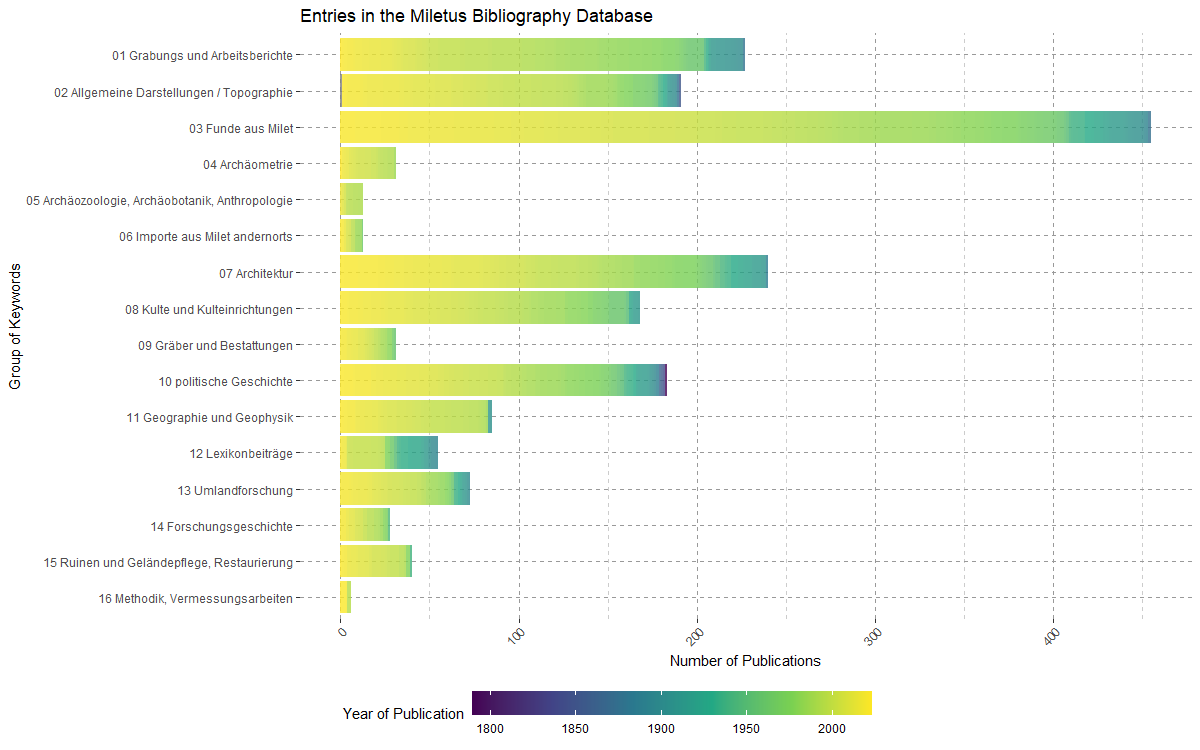
\includegraphics[width=\textwidth]{../figures/mil-pubs-by-keys.png}
\newpage
 
\begin{flushleft}%

\section{Grabungs- und Arbeitsberichte (chronologisch)}%
    
\newrefcontext[sorting=ynt]
\printbibliography[keyword={01 Grabungs und Arbeitsberichte},heading=none, env=compactbib]

\newrefcontext[sorting=nyt]
%\printbibliography[keyword={02 Allgemeine Darstellungen / Topographie},heading=none, env=compactbib]
\section{Allgemeine Darstellungen und Topographie}
\subsection[Prähistorisch]{Topographie: Prähistorisch}
\printbibliography[keyword={02-01 Topographie: Prähistorisch},heading=none, env=compactbib]

\subsection[Bronzezeit]{Topographie: Bronzezeit}
\printbibliography[keyword={02-02 Topographie: Bronzezeit},heading=none, env=compactbib]
\subsection[geometrische Zeit]{Topographie: geometrische Zeit}
\printbibliography[keyword={02-03 Topographie: geometrische Zeit},heading=none, env=compactbib]
\subsection[archaische Zeit]{Topographie: archaische Zeit}
\printbibliography[keyword={02-04 Topographie: archaische Zeit},heading=none, env=compactbib]
\subsection[klassische Zeit]{Topographie: klassische Zeit}
\printbibliography[keyword={02-05 Topographie: klassische Zeit},heading=none, env=compactbib]
\subsection[hellenistische Zeit]{Topographie: hellenistische Zeit}
\printbibliography[keyword={02-06 Topographie: hellenistische Zeit},heading=none, env=compactbib]
\subsection[Kaiserzeit]{Topographie: Kaiserzeit}
\printbibliography[keyword={02-07 Topographie: Kaiserzeit},heading=none, env=compactbib]
\subsection[Spät- und Nachantike]{Topographie: Spät- und Nachantike}
\printbibliography[keyword={02-08 Topographie: Spät und Nachantike},heading=none, env=compactbib]
\subsection[Mittelalter / Balat]{Topographie: Mittelalter / Balat}
\printbibliography[keyword={02-09 Topographie: Mittelalter / Balat},heading=none, env=compactbib]

\section{Funde aus Milet}
%\printbibliography[keyword={03 Funde aus Milet},heading=none, env=compactbib]
\subsection[Gattungsübergreifend]{Funde: Gattungsübergreifend}
\printbibliography[keyword={03-01 Funde: Gattungsübergreifend},heading=none, env=compactbib]
\subsection[Varia]{Funde: Varia}
\printbibliography[keyword={03-02 Funde: Varia},heading=none, env=compactbib]
\subsection[Architekturteile, Bauornamentik]{Funde: Architekturteile, Bauornamentik}
\printbibliography[keyword={03-03 Funde: Bauteile; Bauornamentik},heading=none, env=compactbib]
\subsection[Skulptur]{Funde: Skulptur}
\printbibliography[keyword={03-04 Funde: Skulptur},heading=none, env=compactbib]
\subsection[Keramik]{Funde: Keramik}
%\printbibliography[keyword={03-05 Funde: Keramik},heading=none, env=compactbib]
\subsubsection[Prähistorisch]{Keramik: Prähistorisch}
\printbibliography[keyword={03-05-01 Keramik: Prähistorisch},heading=none, env=compactbib]
\subsubsection[Bronzezeit]{Keramik: Bronzezeit}
\printbibliography[keyword={03-05-02 Keramik: Bronzezeit},heading=none, env=compactbib]
\subsubsection[geometrische Zeit]{Keramik: geometrische Zeit}
\printbibliography[keyword={03-05-03 Keramik: geometrische Zeit},heading=none, env=compactbib]
\subsubsection[archaische Zeit]{Keramik: archaische Zeit}
\printbibliography[keyword={03-05-04 Keramik: archaische Zeit},heading=none, env=compactbib]
\subsubsection[klassische Zeit]{Keramik: klassische Zeit}
\printbibliography[keyword={03-05-05 Keramik: klassische Zeit},heading=none, env=compactbib]
\subsubsection[hellenistische Zeit]{Keramik: hellenistische Zeit}
\printbibliography[keyword={03-05-06 Keramik: hellenistische Zeit},heading=none, env=compactbib]
\subsubsection[Kaiserzeit]{Keramik: Kaiserzeit}
\printbibliography[keyword={03-05-07 Keramik: Kaiserzeit},heading=none, env=compactbib]
\subsubsection[Spät- und Nachantike]{Keramik: Spät- und Nachantike}
\printbibliography[keyword={03-05-08 Keramik: Spät und Nachantike},heading=none, env=compactbib]
\subsubsection[Mittelalter]{Keramik: Mittelalter}
\printbibliography[keyword={03-05-09 Keramik: Mittelalter},heading=none, env=compactbib]
\subsection[Terrakotta]{Funde: Terrakotta}
\printbibliography[keyword={03-06 Funde: Terrakotta},heading=none, env=compactbib]
\subsection[Metalle]{Funde: Metalle}
\printbibliography[keyword={03-07 Funde: Metalle},heading=none, env=compactbib]
\subsection[Inschriften]{Funde: Inschriften}
\printbibliography[keyword={03-08 Funde: Inschriften},heading=none, env=compactbib]
\subsection[Münzen]{Funde: Münzen}
\printbibliography[keyword={03-09 Funde: Münzen},heading=none, env=compactbib]


\section{Archäometrie}
\printbibliography[keyword={04 Archäometrie},heading=none, env=compactbib]

\section{Archäozoologie, Archäobotanik, Anthropologie}
\printbibliography[keyword={05 Archäozoologie; Archäobotanik; Anthropologie},heading=none, env=compactbib]

\section{Importe aus Milet andernorts}
%\printbibliography[keyword={06 Importe aus Milet andernorts},heading=none, env=compactbib]
\subsection[Numismatik (Milesische Münzen)]{Importe aus Milet: Numismatik (Milesische Münzen)}
\printbibliography[keyword={06-01 Numismatik (Milesische Münzen)},heading=none, env=compactbib]
\subsection[Keramik]{Importe aus Milet: Keramik}
\printbibliography[keyword={06-02 Importe aus Milet: Keramik},heading=none, env=compactbib]
\subsection[Varia]{Importe aus Milet: Varia}
\printbibliography[keyword={06-03 Importe aus Milet: Varia},heading=none, env=compactbib]

\section{Architektur}
\subsection[Varia]{Architektur: Varia}
\printbibliography[keyword={07-01 Architektur: Varia},heading=none, env=compactbib]
\subsection[Stadtmauern und Wehranlagen]{Architektur: Stadtmauern und Wehranlagen}
\printbibliography[keyword={07-02 Architektur: Stadtmauern und Wehranlagen},heading=none, env=compactbib]
\subsection[Theater]{Architektur: Theater}
\printbibliography[keyword={07-03 Architektur: Theater},heading=none, env=compactbib]
\subsection[Delphinion]{Architektur: Delphinion}
\printbibliography[keyword={07-04 Architektur: Delphinion},heading=none, env=compactbib]
\subsection[Platzanlagen und angrenzende Bauten]{Architektur: Platzanlagen und angrenzende Bauten}
\printbibliography[keyword={07-05 Architektur: Platzanlagen und angrenzende Bauten},heading=none, env=compactbib]
\subsection[Bouleuterion]{Architektur: Bouleuterion}
\printbibliography[keyword={07-06 Architektur: Bouleuterion},heading=none, env=compactbib]
\subsection[Gymnasia und Thermenanlagen]{Architektur: Gymnasia und Thermenanlagen}
\printbibliography[keyword={07-07 Architektur: Gymnasia und Thermenanlagen},heading=none, env=compactbib]
\subsection[Häfen und maritime Infrastruktur]{Architektur: Häfen und maritime Infrastruktur}
\printbibliography[keyword={07-08 Architektur: Häfen und maritime Infrastruktur},heading=none, env=compactbib]
\subsection[Wohngebäude]{Architektur: Wohngebäude}
\printbibliography[keyword={07-09 Architektur: Wohngebäude},heading=none, env=compactbib]
\subsection[Wasserversorgung]{Architektur: Wasserversorgung}
\printbibliography[keyword={07-10 Architektur: Wasserversorgung},heading=none, env=compactbib]
\subsection[Kirchen, Synagogen, Moscheen]{Architektur: Kirchen, Synagogen, Moscheen}
\printbibliography[keyword={07-11 Architektur: Kirchen; Synagogen; Moscheen},heading=none, env=compactbib]
\subsection[Werkstätten]{Architektur: Werkstätten}
\printbibliography[keyword={07-12 Architektur: Werkstätten},heading=none, env=compactbib]

%\printbibliography[keyword={},heading=none, env=compactbib]

\section{Kulte und Kulteinrichtungen}
\subsection[Varia]{Kulte: Varia}
\printbibliography[keyword={08-01 Kulte: Varia},heading=none, env=compactbib]
\subsection[Apollon Delphinios]{Kulte: Apollon Delphinios}
\printbibliography[keyword={08-02 Kulte: Apollon Delphinios},heading=none, env=compactbib]
\subsection[Heilige Straße zwischen Milet und Didyma]{Kulte: Heilige Straße zwischen Milet und Didyma}
\printbibliography[keyword={08-03 Kulte: Heilige Straße (Milet<>Didyma)},heading=none, env=compactbib]
\subsection[Athena]{Kulte: Athena}
\printbibliography[keyword={08-04 Kulte: Athena},heading=none, env=compactbib]
\subsection[Dionysos]{Kulte: Dionysos}
\printbibliography[keyword={08-05 Kulte: Dionysos},heading=none, env=compactbib]
\subsection[Aphrodite von Oikous]{Kulte: Aphrodite von Oikous}
\printbibliography[keyword={08-06 Kulte: Aphrodite von Oikous},heading=none, env=compactbib]
\subsection[Artemis Kithone]{Kulte: Artemis Kithone}
\printbibliography[keyword={08-07 Kulte: Artemis Kithone},heading=none, env=compactbib]
\subsection[Demeter]{Kulte: Demeter}
\printbibliography[keyword={08-08 Kulte: Demeter},heading=none, env=compactbib]
\subsection[Heroa]{Kulte: Heroa}
\printbibliography[keyword={08-09 Kulte: Heroa},heading=none, env=compactbib]
\subsection[Kaiserkult]{Kulte: Kaiserkult}
\printbibliography[keyword={08-10 Kulte: Kaiserkult},heading=none, env=compactbib]
\subsection[Athena Assesia]{Kulte: Athena Assesia}
\printbibliography[keyword={08-11 Kulte: Athena Assesia},heading=none, env=compactbib]

\section{Gräber und Bestattungen}
\printbibliography[keyword={09 Gräber und Bestattungen},heading=none, env=compactbib]

\section{Politische Geschichte}
\subsection[Bronzezeit]{Geschichte: Bronzezeit}
\printbibliography[keyword={10-01 Geschichte: Bronzezeit},heading=none, env=compactbib]
\subsection[archaische Zeit]{Geschichte: archaische Zeit}
\printbibliography[keyword={10-02 Geschichte: archaische Zeit},heading=none, env=compactbib]
\subsection[klassische Zeit]{Geschichte: klassische Zeit}
\printbibliography[keyword={10-03 Geschichte: klassische Zeit},heading=none, env=compactbib]
\subsection[hellenistische Zeit]{Geschichte: hellenistische Zeit}
\printbibliography[keyword={10-04 Geschichte: hellenistische Zeit},heading=none, env=compactbib]
\subsection[Kaiserzeit]{Geschichte: Kaiserzeit}
\printbibliography[keyword={10-05 Geschichte: Kaiserzeit},heading=none, env=compactbib]
\subsection[Spät- und Nachantike]{Geschichte: Spät- und Nachantike}
\printbibliography[keyword={10-06 Geschichte: Spät und Nachantike},heading=none, env=compactbib]
\subsection[Mittelalter / Balat]{Geschichte: Mittelalter / Balat}
\printbibliography[keyword={10-07 Geschichte: Mittelalter / Balat},heading=none, env=compactbib]
 
\section{Geographie und Geophysik}
\printbibliography[keyword={11 Geographie und Geophysik},heading=none, env=compactbib]


\section{Lexikonbeiträge}
\printbibliography[keyword={12 Lexikonbeiträge},heading=none, env=compactbib]


\section{Umlandforschung}
\printbibliography[keyword={13 Umlandforschung},heading=none, env=compactbib]


\section{Forschungsgeschichte}
\printbibliography[keyword={14 Forschungsgeschichte},heading=none, env=compactbib]


\section{Ruinen- und Geländepflege, Restaurierung}
\printbibliography[keyword={15 Ruinen und Geländepflege; Restaurierung},heading=none, env=compactbib]

\section{Methodik, Vermessungsarbeiten}
\printbibliography[keyword={16 Methodik; Vermessungsarbeiten},heading=none, env=compactbib]
 
\end{flushleft}

%\end{flushleft}
 

 

 




\end{document}